\documentclass[LI,KR]{HSEUniversity}
% Возможные опции: KR или VKR; LI

\title{Применение методов оптимизации нулевого порядка для тонкой настройки мультимодальных больших языковых моделей}
\author{Татаринов Максим Дмитриевич}
\supervisor{канд. комп. н.}{А. В.~Демидовский}
\reviewer{TBD}{П.П.~Петров}

\Year{2025}
\City{Нижний Новгород}

% \Abstract{
% 	Будущая аннотация.
% }
% Ссылка на файл с описание библиографии
\bibliography{library.bib}

%%%%%%%%%%%%%%%%%%%%%%%%%%%%%%%%
%%% ТЕКСТ РАБОТЫ %%%%%%%%%%%%%%%
\begin{document}

% Обязательные элементы оформления: заголовочный слайд, аннотация, оглавление
\maketitle

\chapter*{Введение}

В последние годы наблюдается стремительное развитие крупных языковых моделей (LLM), обладающих способностью понимать и генерировать текст на уровне,
приближенном к человеческому.
Первоначально их использовали преимущественно для обработки текстовой информации,
однако недавно в фокус исследований и приложений оказались мультимодальные модели (MLLM, или MM-LLM),
способные работать не только с текстом, но и с изображениями, видео, аудио и другими типами данных~\cite{llava, llavaonevision}.
%Такие модели открывают новые перспективы для реализации приложений вроде текстового описания изображений,
%генерации видео по запросу, систем текст-в-речь и других (см., например, LLaVA).

Базовые предобученные языковые модели могут не всегда полностью соответствовать требованиям конкретного случая использования.
Адаптация предобученных моделей к специализированным задачам традиционно осуществляется посредством дообучения, или тонкой настройки (fine-tuning).
Дообучение с использованием методов первого порядка, таких как стохастический градиентный спуск (SGD)~\cite{sgd} или Adam~\cite{adam} используется чаще всего.
Однако с увеличением масштабов моделей проблема потребления оперативной памяти становится всё более острой.
Так, \cite{mezo} показывают, что дообучение модели OPT-13B с использованием полного набора параметров или с помощью методов, ориентированных на параметрическую эффективность (PEFT), требует соответственно в 12 и 6 больше памяти, чем режим работы модели в режиме инференса.
Это объясняется необходимостью кэширования активаций во время прямого прохода,
а также хранения градиентов и состояний оптимизатора при обратном распространении ошибки (backpropagation)~\cite{backpropagation}.
Высокая ресурсоёмкость дообучения моделей, связанная с большим потреблением оперативной памяти,
приводит к необходимости использования дорогостоящего оборудования для выполнения тонкой настройки.

В связи с вышеописанными ограничениями активно развиваются методы адаптации, основанные на подходе, не требующем обратного распространения.
К таким методам относится оптимизация нулевого порядка (ZO).
Несмотря на то, что исследования методов нулевого порядка ведутся уже несколько десятилетий~\cite{spsa,rsg}, лишь в последнее время их начали применять для дообучения LLM, что позволило значительно снизить затраты вычислительной памяти.
Так, Memory-Efficient Zeroth-Order Optimizer (MeZO), предложенный \cite{mezo}, демонстрирует использование памяти сопоставимое с режимом инференса.
При этом, существует недостаток исследований, посвящённых применению методов нулевого порядка к мультимодальным языковым моделям и соответствующим им более сложным задачам.

Таким образом, \textbf{актуальность} данного исследования обусловлена высокой требовательностью к памяти традиционных методов дообучения мультимодальных LLM.
Методы оптимизации нулевого порядка позволяют значительно снизить эти затраты, что открывает возможность их адаптации даже на более дешёвом железе.

%\textbf{Целью} настоящей работы является исследование методов эффективного дообучения мультимодальных больших языковых моделей посредством применения оптимизации нулевого порядка,
%а также проведение сравнительного анализа с традиционными методами оптимизации.

\textbf{Целью} настоящей работы является применение оптимизации нулевого порядка для тонкой настройки мультимодальных больших языковых моделей,
а также проведение сравнительного анализа с традиционными методами оптимизации.

Из поставленной цели были сформулированы следующие \textbf{задачи}:
\begin{enumerate}
    \item Провести обзор современных мультимодальных больших языковых моделей и рассмотреть основные архитектурные решения.
    \item Изучить теоретические основы оптимизации нулевого порядка и исследовать особенности их применения для дообучения нейронных сетей.
    \item Реализовать метод нулевого порядка для адаптации мультимодальной модели.
    \item Провести экспериментальное сравнение эффективности методов оптимизации нулевого порядка и традиционных методов дообучения на ряде специализированных датасетов.
    \item Проанализировать полученные результаты, выявив преимущества и недостатки подхода.
\end{enumerate}

\textbf{Объектом} исследования является процесс дообучения предобученных мультимодальных больших языковых моделей для решения специализированных задач.

\textbf{Предметом} исследования являются реализация и применение методов оптимизации нулевого порядка для эффективной тонкой настройки мультимодальных моделей с минимальными затратами памяти.

Для решения поставленных задач будут использованы следующие \textbf{методы}:
\begin{enumerate}
    \item  Метод анализа и синтеза для создания теоретической базы для данного исследования на основе литературы,
    \item  Методы программирования для написания алгоритмов программы и обучения модели,
    \item  Методы нулевого порядка для оптимизации параметров модели без использования обратного распространения ошибки,
    \item  Методы глубокого обучения для дообучения мультимодальных языковых моделей на специализированных датасетах.
\end{enumerate}

\textbf{Новизна} настоящей работы состоит в том, что в ней рассматривается применение методов оптимизации нулевого порядка к тонкой настройке мультимодальных больших языковых моделей
по сравнению с традиционными методами.

%\textbf{Практическая значимость} данной работы заключается в том, что X.

Работа организована следующим образом:
в первой главе рассматриваются теоретические аспекты мультимодальных больших языковых моделей, а также методы их тонкой настройки;
во второй главе кратко описывается постановка задачи;
в третьей главе приводятся результаты вычислительных экспериментов и их анализ.
В заключении содержатся выводы о проделанной работе.

\chapter{Теория}

\section{Мультимодальные большие языковые модели}

В последние годы большие языковые модели (Large Language Models, LLM) стали одной из центральных тем в области искусственного интеллекта (ИИ).
Их популярность резко возросла благодаря способности генерировать и понимать текст на уровне, близком к человеческому.
Начало этому тренду положил выпуск ChatGPT в 2022 году, который привлек внимание как научного сообщества, так и широкой общественности.
LLM, основанные на архитектуре Transformer, такие как серия GPT от OpenAI (начиная с GPT-1 в 2018 году)~\cite{gpt3}, Google Gemini/BARD, Anthropic CLAUDE и открытые модели,
такие как LLaMA от Meta~\cite{llava} или PaLM от Google~\cite{palm}, продемонстрировали свою универсальность в задачах обработки текста, включая генерацию текста, суммирование, машинный перевод и создание контента в рамках генеративного ИИ.
Однако с развитием технологий и ростом объема данных стало очевидно, что одномодальные системы, работающие исключительно с текстом, не способны полностью удовлетворить потребности сложных реальных задач.

На этом фоне возникли мультимодальные большие языковые модели (Multimodal Large Language Models, MLLM)~\cite{mllm-review}, которые расширяют возможности LLM, интегрируя обработку данных различных типов, таких как текст, изображения, видео и аудио.
MLLM представляют собой значительный шаг вперед в развитии ИИ, поскольку позволяют создавать более полное и точное представление информации за счет синергии между различными модальностями.
Это открывает новые горизонты для приложений, таких как генерация описаний изображений (image captioning), создание видео по текстовым запросам, обработка аудио с учетом контекста и многие другие.
В отличие от традиционных одномодальных систем, MLLM способны не только анализировать данные отдельно по каждой модальности, но и находить сложные взаимосвязи между ними, что делает их незаменимыми для задач, требующих комплексного мультимодального анализа.

\subsubsection*{Исторический контекст и развитие MLLM}

История развития MLLM берет начало с попыток объединить достижения в области компьютерного зрения и обработки естественного языка (Natural Language Processing, NLP).
Ранние подходы к мультимодальной обработке информации были вдохновлены методами машинного перевода.
В таких системах изображение сначала преобразовывалось в промежуточное представление с помощью сверточной нейронной сети (CNN), а затем это представление передавалось в рекуррентную нейронную сеть (RNN) для генерации текстового описания~\cite{imagecaptioningdeeplearning}.
Однако такие методы были вычислительно затратными и часто давали неточные результаты.
Со временем исследователи начали искать более эффективные способы интеграции модальностей.

Одним из ключевых прорывов стало появление модели Contrastive Language-Image Pre-training (CLIP)~\cite{clip}, представленной в 2021 году.
CLIP, обученная на 400 миллионах пар изображений и текстов, продемонстрировала способность к zero-shot классификации,
то есть могла выполнять задачи без дополнительного обучения на конкретных данных.
Этот подход стал основой для многих современных MLLM, поскольку позволил эффективно сопоставлять визуальные и текстовые представления.
BLIP-2~\cite{blip2}, представленный в 2023 году, продемонстрировал подход к объединению визуальных и текстовых представлений через двухэтапное обучение.
В нём Querying Transformer (Q-Former) извлекает ключевые визуальные особенности из заранее обученного и неизменяемого кодировщика изображений,
а затем адаптирует их для взаимодействия с замороженной языковой моделью, обеспечивая тем самым более глубокое и точное сопоставление между изображениями и текстом.

\subsubsection*{Примеры современных MLLM}

Среди современных MLLM можно выделить несколько ключевых моделей, которые демонстрируют разнообразие подходов к интеграции модальностей.
LLaVA (Large Language and Vision Assistant)~\cite{llava}, представленная в 2023 году, сочетает визуальный энкодер CLIP с языковой моделью Vicuna для общего понимания связи между изображениями и текстом.
Эта модель была дообучена на наборе данных MS-COCO, что позволило ей эффективно обрабатывать задачи, связанные с визуально-языковым взаимодействием.
LLaVA 1.5 добавила улучшения в виде более мощного энкодера CLIP-ViT-L и проекционного слоя на основе многослойного перцептрона (MLP), что повысило ее точность.

MiniGPT4~\cite{minigpt4}, разработанная в 2023 году исследователями из KAUST, представляет собой открытую альтернативу GPT-4 от OpenAI.
Эта модель использует замороженные визуальные компоненты (Q-Former и ViT) и языковую модель Vicuna, соединяя их с помощью одного проекционного слоя.
%MiniGPT4 показала впечатляющие результаты в задачах интерпретации мемов, генерации рецептов и создания рекламного контента, превосходя BLIP-2 по многим метрикам, хотя и страдает от типичных для LLM проблем, таких как галлюцинации.

mPLUG-OWL\cite{mplugowl}, представленная в 2023 году исследователями из Alibaba DAMO Academy, предлагает новый подход к выравниванию изображений и текста, замораживая визуальную модель только на втором этапе обучения.
Используя LLaMA-7B как языковую модель и ViT-L/14 как визуальный энкодер, mPLUG-OWL демонстрирует высокую производительность в задачах визуального понимания, хотя также сталкивается с проблемами галлюцинаций.

Семейство открытых мультимодальных моделей LLaVA-OneVision~\cite{llavaonevision}, представленное в конце 2024 года, справляется с обработкой одиночных изображений,
мультизвуковых последовательностей и видеосигналов
Архитектура модели объединяет в себе следующие компоненты:
языковую модель Qwen-2,
визуальный энкодер SigLIP, обеспечивающий извлечение признаков изображений и видео,
и двухслойный MLP-проектор для проекции визуальных признаков в языковое пространство эмбеддингов.
Экспериментальные результаты демонстрируют, что подход обеспечивает переносимость знаний между различными сценариями, что подтверждается успешным применением модели в рамках задач видеоанализа и кросс-модального обучения.

\subsection*{Устройство мультимодальных языковых моделей}

\begin{figure}[H]
\centering
\begin{tikzpicture}[
    % Adjusted node style for the large box
    box/.style={
        rectangle,
        rounded corners,
        draw,
        drop shadow,
        fill=#1!20,
        text width=12cm,
        align=center,
        minimum height=3em,
        inner sep=2mm
    },
    % Adjusted node style for the smaller box
    box-small/.style={
        rectangle,
        rounded corners,
        draw,
        drop shadow,
        fill=#1!20,
        text width=5cm,
        align=center,
        minimum height=3em,
        inner sep=2mm
    },
    % Adjusted arrow style
    arrow/.style={
        semithick,              % Lighter line than "thick"
        -{Stealth[scale=0.8]},  % Smaller arrowhead than scale=1.2
        draw=#1
    },
    label/.style={
        font=\footnotesize
    }
]

    % Define Colors
    \definecolor{inputcolor}{RGB}{135,206,250}    % Light Sky Blue
    \definecolor{modelcolor}{RGB}{144,238,144}      % Light Green
    \definecolor{outputcolor}{RGB}{255,182,193}     % Light Pink

    \node (output) {
    \small Языковой ответ ($Xa$)
    };
    % Nodes with slightly reduced text sizes
    \node[box=inputcolor, below=0.35cm of  output] (languagemodel) {
    \small \textbf{Языковая модель}
    };

    \node (visualtokens)
    [below=0.35cm of  languagemodel, xshift=-3.5cm] {
        \small Визуальные токены ($Hv$)
    };
    \node[box-small=modelcolor, below=0.35cm of  visualtokens] (projection) {
        \small \textbf{Проектор}
    };

    \node (visualfeatures)
    [below=0.35cm of  projection] {
        \small Визуальные признаки ($Zv$)
    };
    \node[box-small=outputcolor, below=0.35cm of  visualfeatures] (visionencoder) {
        \small \textbf{Кодировщик изображений}
    };

    \node (visualsignal)
    [below=0.35cm of  visionencoder] {
        \small Входное изображение ($Xv$)
    };

    \node (languageinstruction)
    [below=0.35cm of  languagemodel, xshift=3.5cm] {
        \small Языковая инструкция ($Xq$)
    };
    % Arrows with labels in a smaller font

    \draw[arrow=black] (languagemodel) -- (output);
    \draw[arrow=black] (visualtokens) -- (languagemodel);
    \draw[arrow=black] (projection) -- (visualtokens);
    \draw[arrow=black] (visualfeatures) -- (projection);
    \draw[arrow=black] (visionencoder) -- (visualfeatures);
    \draw[arrow=black] (visualsignal) -- (visionencoder);
    \draw[arrow=black] (languageinstruction) -- (languagemodel);

\end{tikzpicture}
\caption{Архитектура MLLM}
\label{fig:mllm-structure}
\end{figure}

Популярная схема устройства MLLM включает три основных блока~\cite{llavaonevision, llava}:

\textbf{1. Визуальный энкодер}.
Для анализа изображений применяется визуальный энкодер, который преобразует входное изображение ($Xv$) в набор визуальных признаков ($Zv$).
Такие признаки могут быть извлечены как из промежуточных слоёв трансформера, так и из его финальных слоёв,
что обеспечивает учёт пространственного расположения элементов и глубину представления.

\textbf{2. Проектор}.
Специальная проекционная сеть играет ключевую роль в объединении текстовых и визуальных представлений.
Обычно для этой цели используется лёгкий модуль (например, двухслойный MLP или простая линейная трансформация),
который отображает визуальные признаки ($Zv$) в то же пространство эмбеддингов, что и текстовые представления языковой модели.
Итогом является формирование последовательности «визуальных токенов» ($Hv$), сопоставимых с текстовыми.

\textbf{3. Языковая модель}.
В основе системы лежит языковая модель, предобученная на огромном корпусе текстов, такие как Vicuna или Qwen-2.
Она отвечает за генерацию ответов и формирование связного текста.
Языковая модель принимает на вход как текстовые инструкции ($Xq$), так и визуальные токены ($Hv$), объединяя их для генерации ответа ($Xa$).
%Выбор конкретного LLM определяется требуемыми характеристиками генеративной мощности и способностью к точному следованию инструкциям.

Обучение мультимодальных моделей является многоэтапным процессом, направленным на выравнивание представлений разных модальностей и адаптацию модели к конкретным задачам.

1. Первоначальным этапом является выравнивание представлений между модальностями.
На этом этапе замораживаются веса как визуального энкодера, так и языковой модели, а обучается только проекционный слой.
Это позволяет эффективно преобразовать визуальные данные в формат, совместимый с языковой моделью, поскольку визуальные токены приводятся в форму,
максимально приближенную к распределению текстовых эмбеддингов.

2. После этого начинается основной этап обучения, в рамках которого как правило уже все компоненты модели (в том числе LLM, визуальный энкодер и проектор) подвергаются дообучению.
На данном этапе задача заключается в тонкой настройке модели, чтобы она могла эффективно связывать информацию из изображения с текстовыми запросами.
При этом обучающие примеры могут варьироваться от простых описаний изображений до более сложных многозадачных сценариев, что содействует появлению «новых» способностей в рамках мультимодального взаимодействия. Размер и сложность входных данных постепенно увеличиваются, что позволяет модели адаптироваться к обработке изображений более высокого разрешения и большему числу визуальных токенов без резкого скачка вычислительной нагрузки.

\section{Тонкая настройка языковых моделей и её методы}

Потенциал, предоставляемый заранее обученными LLM и MLLM, огромен.
Однако эти базовые модели не всегда могут идеально соответствовать специфическим требованиям каждого конкретного случая использования.
В некоторых случаях может требоваться более персонализированный вывод, а в других – отсутствует важный контекст или специализированные знания,
которые не были получены на этапе первоначального обучения.
Чтобы в полной мере использовать потенциал заранее обученных базовых моделей для конкретных случаев применения,
можно прибегнуть к тонкой настройке модели (файн-тьюнинг, от англ. fine-tuning).

Тонкая настройка – это процесс изменения некоторых параметров заранее обученной базовой модели путем дальнейшего обучения на меньшем, специализированном для определенной задачи наборе данных с целью оптимизировать производительность модели для конкретного случая.
Полная тонкая настройка предполагает корректировку всех параметров заранее обученной модели на специализированном наборе данных,
чтобы модель лучше соответствовала специфическим требованиям целевого случая использования.
Хотя такой подход обеспечивает всестороннюю настройку, он требует значительного объема обучающих данных.
Преимущество полной тонкой настройки заключается в способности модели улавливать тонкости конкретной области,
однако этот процесс может быть вычислительно затратным~\cite{mezo}.
В связи с этим, в последние годы наблюдается рост интереса к методам тонкой настройки, которые требуют меньшего объема вычислительных ресурсов и памяти.

%\section*{Путь к Memory-Efficient Zeroth-Order Optimizer (MeZO)}

Методы параметрически-эффективной тонкой настройки (Parameter-Efficient Fine-Tuning, PEFT), например LoRA~\cite{lora}, обновляют лишь небольшую часть параметров модели. %ZeRA~\cite{rajbhandari2020}, EMAT~\cite{wu2022} и другие
Хотя такие подходы позволяют дообучать большие языковые модели (LLM) при относительно низких затратах памяти и вычислительных ресурсов,
в определённых случаях более предпочтительной оказывается полная тонкая настройка, позволяющая задействовать всю модель~\cite{fullpeftcomparison}.

В условиях ограниченных вычислительных ресурсов важным становится использование методов полной тонкой настройки с низким потреблением памяти.
Так, подход \emph{Low-Memory Optimization (LOMO)}~\cite{adalomo} отказывается от хранения градиентов при использовании стохастического градиентного спуска (SGD)~\cite{sgd, sgd-analysis}, однако градиенты вычисляются на каждом шаге обучения.
Альтернативой является оптимизация нулевого порядка (Zeroth-Order Optimization, ZO), которая позволяет оценивать градиенты, используя только прямые проходы через модель.
Такой подход требует объёма памяти, сопоставимого с режимом инференса.

В работе \cite{mezo} предложен \emph{Memory-Efficient Zeroth-Order Optimizer (MeZO)} для дообучения LLM исключительно на основе прямых проходов без обратного распространения ошибки.
Достижение высоких результатов MeZO объясняется тем, что в предобученных глубоких нейронных сетях матрицы Гессе обладают небольшим локальным эффективным рангом~\cite{hessianrank1, hessianrank2, hessianrank3}.
Метод вычисляет оценку градиента всего за два прямых прохода, используя рандомизированное возмущение параметров, что существенно снижает задержки между вычислениями на GPU по сравнению с методами типа LOMO.

\subsection{Оптимизация нулевого порядка (ZO)}\label{subsec:ZO}
Оптимизация нулевого порядка давно изучается в задачах выпуклой и сильно выпуклой оптимизации.
В качестве классического оценивателя градиента используется метод одновременного стохастического приближения с возмущениями (Simultaneous Perturbation Stochastic Approximation, SPSA)~\cite{spsa}.
Он позволяет заменить вычисление градиента в традиционном SGD на оценку, основанную исключительно на прямых проходах.

Рассмотрим размеченный датасет
$
\mathcal{D} = \{(x_i, y_i)\}_{i\in|\mathcal{D}|},
$
мини-батч
$
\mathcal{B} \subset \mathcal{D},
$
размера $B$ и функцию потерь $\mathcal{L}(\theta; \mathcal{B})$ для модели с параметрами $\theta \in \mathbb{R}^d$.
Тогда оценка градиента методом SPSA определяется следующим образом:
$$
\widehat{\nabla} \mathcal{L}(\theta; \mathcal{B}) = \frac{\mathcal{L}(\theta + \epsilon z; \mathcal{B}) - \mathcal{L}(\theta - \epsilon z; \mathcal{B})}{2\epsilon}\, z.
$$
%что можно записать и в виде приближения:
%$$
%\widehat{\nabla} \mathcal{L}(\theta; \mathcal{B}) \approx zz^\top \nabla \mathcal{L}(\theta; \mathcal{B}).
%$$
Здесь $z \in \mathbb{R}^d$ выбирается из нормального распределения, $z \sim \mathcal{N}(0, I)$, где $I$ — единичная матрица, а $\epsilon$ представляет масштаб возмущения.

Метод SPSA требует всего двух прямых проходов через модель для оценки градиента, после чего полученная оценка используется для обновления параметров по схеме:
$$
\theta_{t+1} = \theta_t - \eta\, \widehat{\nabla} \mathcal{L}(\theta; \mathcal{B}_t),
$$
где $\mathcal{B}_t$ — мини-батч на шаге $t$, а $\eta$ — скорость обучения.

\subsection{MeZO}

Алгоритм ZO-SGD в классической реализации требует вдвое больше памяти, чем при инференсе, из-за необходимости хранить вектор $z \in \mathbb{R}^d$.
В работе \cite{mezo} предложена память-эффективная версия этого алгоритма, названная MeZO.
Имплементация представлена в виде алгоритма~\ref{alg:mezo}.
На каждом шаге генерируется случайное начальное значение $s$, которое используется для сброса генератора случайных чисел и повторной выборки нужных элементов $z$ при каждом из четырех применений в алгоритме.
Такая реализация «на месте» позволяет MeZO сократить объем памяти до уровня, эквивалентного затратам на инференс.

Кроме того, авторами отмечается, что раздельное возмущение каждого параметра может быть слишком затратным по времени для больших моделей.
В практической реализации предлагается возмущать целые весовые матрицы вместо отдельных скаляров, что ускоряет обучение,
но увеличивает необходимый объем памяти на размер крупнейшей матрицы, например на размер матрицы словарных эмбеддингов для OPT-66B (0.86 ГБ).

\begin{algorithm}[H]
\caption{MeZO}
\begin{algorithmic}[1]
\Require параметры модели $\theta \in \mathbb{R}^d$, функция потерь $\mathcal{L} : \mathbb{R}^d \rightarrow \mathbb{R}$, количество шагов $T$, масштаб возмущения $\epsilon$, размер батча $B$, скорость обучения $\eta_t$
\For{$t = 1, \ldots, T$}
    \State Выбрать батч $\mathcal{B} \subset \mathcal{D}$ и случайный сид $s$
    \State $\theta \leftarrow \text{ВозмущениеПараметров}(\theta, \epsilon, s)$
    \State $\ell_+ \leftarrow \mathcal{L}(\theta; \mathcal{B})$
    \State $\theta \leftarrow \text{ВозмущениеПараметров}(\theta, -2\epsilon, s)$
    \State $\ell_- \leftarrow \mathcal{L}(\theta; \mathcal{B})$
    \State $\theta \leftarrow \text{ВозмущениеПараметров}(\theta, \epsilon, s)$ \Comment{Возврат параметров к исходному состоянию}
    \State $\text{projected\_grad} \leftarrow (\ell_+ - \ell_-)/(2\epsilon)$
    \State Сбросить генератор случайных чисел с сидом $s$ \Comment{Для выборки $z$}
    \ForAll{$\theta_i \in \theta$}
        \State $z \sim \mathcal{N}(0, 1)$
        \State $\theta_i \leftarrow \theta_i - \eta_t \cdot \text{projected\_grad} \cdot z$
    \EndFor
\EndFor
\end{algorithmic}
\label{alg:mezo}
\end{algorithm}

\begin{algorithm}[H]
\caption{ВозмущениеПараметров}
\begin{algorithmic}[1]
\Require $\theta, \epsilon, s$
\State Сбросить генератор случайных чисел с сидом $s$ \Comment{Для выборки $z$}
\ForAll{$\theta_i \in \theta$}
    \State $z \sim \mathcal{N}(0, 1)$
    \State $\theta_i \leftarrow \theta_i + \epsilon \cdot z$ \Comment{Изменение параметров на месте}
\EndFor
\State \Return $\theta$
\end{algorithmic}
\end{algorithm}

Кроме минимального использования памяти во время обучения,
преимуществом MeZO является возможность сохранять чекпойнты,
включающие только сид $s$ и оценку градиента.
Такой чекпойнт позволяет восстановить состояние модели из изначальных параметров, но
занимая значительно меньше места, чем традиционные чекпойнты, содержащие веса модели.

Недостатками MeZO согласно \cite{mezo} является то, что
для достижения хорошей производительности требуется большое количество итераций,
а также грамотно составленный промпт, так как метод работает только в тех условиях,
когда траектория оптимизации ведет себя достаточно благоприятсвующе.

Среди попыток улучшить MeZO можно выделить MeZO-SVRG~\cite{mezo-svrg}, в котором происходит уменьшение дисперсии оценок градиента,
однако MeZO-SVRG потребляет больше памяти, чем MeZO, из-за необходимости хранения копий параметров и оценок градиента, рассчитанных на полный батч.

\section*{Выводы}

Таким образом, в настоящее время разрабатывается множество мультимодальных больших языковых моделей MLLM, которые состоят из визуального энкодера, проекционного слоя и языковой модели.
Вначале при разработке таких моделей обучается проекционный слой, обеспечивающий выравнивание визуальных и текстовых представлений,
а затем производится адаптация различных компонентов модели – от отдельно языковой модели до полной архитектуры с визуальным энкодером.
Традиционные методы тонкой настройки, такие как Adam, требуют значительных затрат памяти из-за необходимости вычисления градиентов через обратное распространение ошибки.
Алгоритмы нулевого порядка, такие как MeZO, демонстрируют потенциал значительного уменьшения использования памяти и могут быть применены для оптимизации MLLM.

\chapter{Постановка задачи}

В данной работе рассматривается задача тонкой настройки предобученных мультимодальных больших языковых моделей (MLLM) с использованием методов оптимизации нулевого порядка (ZO, см. раздел~\ref{subsec:ZO}), что позволяет значительно сократить потребление памяти по сравнению с традиционными методами, такими как AdamW~\cite{adam, adamw}.

\textbf{Этап 1. Подготовка и формулировка задачи.} Пусть имеется предобученная мультимодальная языковая модель $ M $ с параметрами $ \theta \in \mathbb{R}^{d} $, способная обрабатывать как текстовую, так и визуальную информацию.
В качестве обучающих данных используется выборка $D = \{(I_i, T_i, Y_i)\}_{i=1}^{N}$,
которая охватывает несколько уровней сложности и типов задач, где:
\begin{itemize}
    \item $ I_i $ – изображение, представляющее визуальную информацию;
    \item $ T_i $ – текстовый промпт, содержащий текстовую информацию;
    \item $ Y_i = (y_{i1}, y_{i2}, \dots, y_{iL'_i}) $ – требуемый эталонный ответ (последовательность токенов).
\end{itemize}

\textbf{Этап 2. Имплементация метода и дообучение.} Данная часть состоит в адаптации существующего пайплайна обучения модели $ M $ для интеграции алгоритма нулевого порядка MeZO, что требует переписывания части обучающей логики, а также проведения сравнения с традиционными методами настройки.
Так, в алгоритме MeZO для датасета
$$
\mathcal{D} = \{(x_i, y_i)\}_{i=1}^{|\mathcal{D}|},
$$
для мини-батча $ \mathcal{B} \subset \mathcal{D} $ размера $ B $ и функции потерь $ \mathcal{L}(\theta; \mathcal{B}) $ для модели с параметрами $ \theta \in \mathbb{R}^{d} $ оценка градиента производится следующим образом:
$$
\widehat{\nabla} \mathcal{L}(\theta; \mathcal{B}) = \frac{\mathcal{L}(\theta + \epsilon z; \mathcal{B}) - \mathcal{L}(\theta - \epsilon z; \mathcal{B})}{2\epsilon}\, z,
$$
где $ \epsilon > 0 $ – величина пертурбации, а $ z \in \mathbb{R}^{d} $ – случайный вектор.
Подробное описание метода приведено в алгоритме~\ref{alg:mezo}.

При тонкой настройке модели применяется метод принудительного обучения (teacher forcing).
Функция потерь определяется как кросс-энтропия между логитами, генерируемыми языковой моделью, и истинным ответом.
Более формально, если $Y_i = (y_{i1}, y_{i2}, \dots, y_{iL'_i})$ – эталонная последовательность токенов,
то функция потерь записывается как
$$
L(\theta) = - \sum_{i=1}^{N} \sum_{j=1}^{L'_i} \log p\Bigl(y_{ij} \,\bigl|\, I_i,\, T_i,\; y_{i1}, \dots, y_{i,j-1};\, \theta\Bigr).
$$
При этом токены, относящиеся к первоначальному промпту, исключаются из суммирования.

На этапе инференса для формирования ответа используется жадное декодирование:
$$
\hat{y}_{ij} = \arg\max_{k}\, p\Bigl(k \,\bigl|\, I_i,\, T_i,\; \hat{y}_{i1}, \dots, \hat{y}_{i,j-1};\, \theta\Bigr).
$$

\textbf{Этап 3. Экспериментальное сравнение и оценка.} Для оценки эффективности предлагаемого метода планируется проведение сравнительного анализа по следующим направлениям:
\begin{enumerate}
    \item \textbf{Качество дообучения.} Оценка точности генерируемых ответов для каждого датасета при использовании разных конфигураций модели:
дообучение только языковой модели (LM); дообучение в комбинации с проекционным слоем (LM+Projector); дообучение всей архитектуры (LM+Projector+Vision Encoder).
    В качестве эталонного сравнения используются результаты дообучения методом AdamW.
    \item \textbf{Сходимость и стабильность обучения.} Анализ кривых функции потерь, выявление особенностей сходимости и устойчивости оптимизационного процесса.
    \item \textbf{Потребление памяти.} Измерение пикового использования памяти для каждого подхода.
\end{enumerate}

\section{Модель}

В качестве мультимодальной большой языковой модели для экспериментов используется LLaVA-OneVision~\cite{llavaonevision},
а именно llava-onevision-qwen2-0.5b-si (версия с 0.5B параметров) и llava-onevision-qwen2-7b-si (версия с 7B параметров).
Версия Single-Image (SI) выбрана, так как набор датасетов, используемый в настоящей работе, сфокусирован на одиночных изображениях, и подразумевает, что модель предобучена на обработку одиночных изображений, а не на видео.
Архитектура LLaVA-OneVision представлена на рисунке~\ref{fig:llava-onevision-structure}.

\begin{figure}[H]
\centering
\begin{tikzpicture}[
    box/.style={
        rectangle,
        rounded corners,
        draw,
        drop shadow,
        fill=#1!20,
        text width=12cm,
        align=center,
        minimum height=3em,
        inner sep=2mm
    },
    box-small/.style={
        rectangle,
        rounded corners,
        draw,
        drop shadow,
        fill=#1!20,
        text width=5cm,
        align=center,
        minimum height=3em,
        inner sep=2mm
    },
    arrow/.style={
        semithick,
        -{Stealth[scale=0.8]},
        draw=#1
    },
    label/.style={
        font=\footnotesize
    }
]

    \definecolor{inputcolor}{RGB}{135,206,250}    % Light Sky Blue
    \definecolor{modelcolor}{RGB}{144,238,144}      % Light Green
    \definecolor{outputcolor}{RGB}{255,182,193}     % Light Pink

    \node (output) {
    \small Языковой ответ ($Xa$)
    };

    \node[box=inputcolor, below=0.35cm of  output] (languagemodel) {
    \small \textbf{Qwen-2}
    };

    \node (visualtokens)
    [below=0.35cm of  languagemodel, xshift=-3.5cm] {
        \small Визуальные токены ($Hv$)
    };
    \node[box-small=modelcolor, below=0.35cm of  visualtokens] (projection) {
        \small \textbf{MLP Projector}
    };

    \node (visualfeatures)
    [below=0.35cm of  projection] {
        \small Визуальные признаки ($Zv$)
    };
    \node[box-small=outputcolor, below=0.35cm of  visualfeatures] (visionencoder) {
        \small \textbf{SigLIP Encoder}
    };

    \node (visualsignal)
    [below=0.35cm of  visionencoder] {
        \small Входное изображение ($Xv$)
    };

    \node (languageinstruction)
    [below=0.35cm of  languagemodel, xshift=3.5cm] {
        \small Языковая инструкция ($Xq$)
    };

    \draw[arrow=black] (languagemodel) -- (output);
    \draw[arrow=black] (visualtokens) -- (languagemodel);
    \draw[arrow=black] (projection) -- (visualtokens);
    \draw[arrow=black] (visualfeatures) -- (projection);
    \draw[arrow=black] (visionencoder) -- (visualfeatures);
    \draw[arrow=black] (visualsignal) -- (visionencoder);
    \draw[arrow=black] (languageinstruction) -- (languagemodel);

\end{tikzpicture}
\caption{Архитектура LLaVA-OneVision}
\label{fig:llava-onevision-structure}
\end{figure}

\section{Датасеты}

Набор датасетов представлен разными задачами различной сложности.

Br35H - это классификационный датасет, содержащий 3000 изображений MRI мозга, поровну разделённых на 2 класса: здоровые и с опухолями.

\begin{table}[H]
\centering
\begin{tabular}{| m{4cm} | m{10cm} |}
\hline
\textbf{Ключ} & \textbf{Содержание} \\ \hline
Изображение & 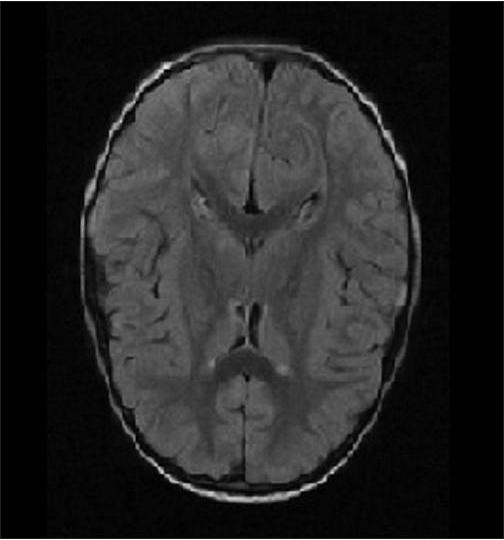
\includegraphics[scale=0.15]{images/br35h_example} \\ \hline
Ответ & No \\ \hline
\end{tabular}
\caption{Пример вхождения в датасет Br35H}
\end{table}

We-Math - это бенчмарк с задачей множественного выбора, содержащий 1740 визуальных математических проблем~\cite{wemath}.
Каждый пример состоит из изображения математической задачи, текстового вопроса и 5 вариантов ответа, из которых только один правильный.

\begin{table}[H]
\centering
\begin{tabular}{| m{4cm} | m{12cm} |}
\hline
\textbf{Ключ} & \textbf{Содержание} \\ \hline
Изображение & 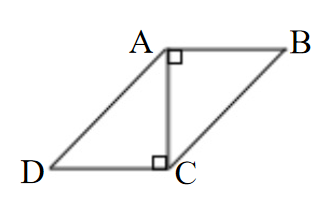
\includegraphics[scale=0.35]{images/wemath_example} \\ \hline
Вопрос & As shown in the diagram, two identical isosceles right triangles are combined to form a parallelogram. The perimeter is reduced by 20 cm. What is the length of AB=AC= ( ) cm? \\ \hline
%Варианты ответа & A. 10 cm; B. 20 cm; C. 5 cm; D. 4 cm; E. No correct answer \\ \hline
%Ответ & A \\ \hline
Варианты ответа & 10 cm; 20 cm; 5 cm; 4 cm; No correct answer \\ \hline
Ответ & 10 cm \\ \hline
\end{tabular}
\caption{Пример вхождения в датасет We-Math}
\end{table}

ChartQA - это бенчмарк, включающий 9,6 тысяч вопросов, написанных человеком,
а также 23,1 тысыч вопросов, сгенерированных на основе описаний диаграмм, написанных человеком~\cite{chartqa}.
Каждый пример состоит из изображения графика или диаграммы, текстового вопроса и правильного ответа.

\begin{table}[H]
\centering
\begin{tabular}{| m{4cm} | m{12cm} |}
\hline
\textbf{Ключ} & \textbf{Содержание} \\ \hline
Изображение & 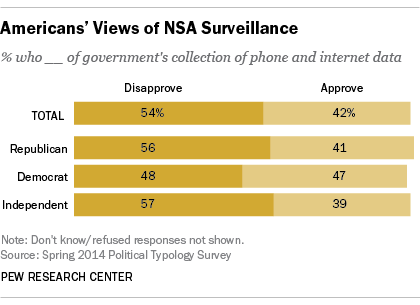
\includegraphics[scale=0.6]{images/chartqa_example} \\ \hline
Вопрос & Which party is least likely to approve NSA surveillance? \\ \hline
Ответ & Independant \\ \hline
\end{tabular}
\caption{Пример вхождения в датасет ChartQA}
\end{table}

\chapter{Вычислительные эксперименты}

Аналогично \cite{mezo} для датасетов создавались обучающие выборки, состоящие из 1000 примеров, тестовые выборки, состоящие из 1000 примеров, и валидационные из 500.
В случае недостатка примеров в датасете, тестовая и валидационная выборки были созданы из меньшего количества примеров.
Если в датасете не было разделения на обучающую и тестовую выборки, то они были созданы случайным образом.
Изображения были приведены к размеру 384x384 пикселей (равноценно 729 визуальным токенам), если превышали это разрешение.

Для модели LLaVA-OneVision-Qwen2-0.5B-SI запуски проводились на NVIDIA RTX 3090 24GB.
Для модели LLaVA-OneVision-Qwen2-7B-SI запуски проводились на NVIDIA A100 80GB.

Если не указано иное, использовались следующие гиперпараметры:

\begin{table}[H]
\centering
\begin{tabular}{|l|c|}
\hline
Параметр & Значение \\ \hline
Шаг обучения (learning rate) & 1e-6 \\ \hline
Весовое затухание (weight decay) & 0.0 \\ \hline
bfloat16 & Да \\ \hline
Степень пертубации (zo\_eps) & 0.001 \\ \hline
Планировщик скорости обучения (learning rate scheduler) & Постоянный (constant) \\ \hline
\end{tabular}
\caption{Параметры запуска MeZO и AdamW}
%\label{tab:mezo-prompt-engineering-parameters}
\end{table}

Для экспериментов с AdamW использовался размер батча 1 и 3000 шагов обучения.
Для экспериментов с MeZO использовался размер батча 4.
Из-за сообщаемой в \cite{mezo} меньшей скорости сходимости MeZO, количество шагов обучения было увеличено до 5000.

Более подробный список гиперпараметров приведён в приложении~\ref{app:mezo-parameters}.

\section{Подготовка промптов}

Так как качество MeZO сильно зависит от качества постановки промпта~\cite{mezo},
то изначально мы рассматриваем несколько вариантов шаблона промпта, который может быть использован,
тестируя их после обучения в течение одной эпохи (250 шагов) на датасете \textit{Br35H}.

\begin{itemize}[leftmargin=10mm]
    \item Промпт 1:\\
    \small{\texttt{<image>}\textbackslash n\texttt{Question: Are there signs of a tumor in the image? Yes or No?}\textbackslash n\texttt{Answer:}\textbackslash s}

    \item Промпт 2:\\
    \small{\texttt{<image>}\textbackslash n\texttt{Question: Are there signs of a tumor in the image? Yes or No?}\textbackslash n\texttt{Answer:}}

    \item Промпт 3:\\
    \small{\texttt{<image>}\textbackslash n\texttt{Question: Are there signs of a tumor? Yes or No?}\textbackslash n\texttt{Answer:}}

    \item Промпт 4:\\
    \small{\texttt{<image>}\textbackslash n\texttt{Question: Are there signs of a tumor in the image? Yes or No?}}

    \item Промпт 5:\\
    \small{\texttt{<image>}\textbackslash n\texttt{Are there signs of a tumor in the image? Yes or No?}\textbackslash n\texttt{Answer:}}

    \item Промпт 6:\\
    \small{\texttt{<image> Are there signs of a tumor in the image? Yes or No? Answer:}}

    \item Промпт 7:\\
    \small{\texttt{<image>}\textbackslash n\texttt{Are there signs of a tumor in the image? Respond with Yes or No.}\textbackslash n\texttt{Answer:}}
\end{itemize}

Так, результаты тестирования различных промптов для датасета \textit{Br35H} представлены в таблице~\ref{tab:prompt-engineering-results}.

\begin{table}[H]
\centering
\begin{tabular}{|l|c|c|}
\hline
\textbf{Промпт} & \textbf{Zero-shot (\%)} & \textbf{MeZO (\%)} \\ \hline
Промпт 1 & 61.1 & 78.2 \\ \hline
Промпт 2 & 66.0 & 52.3 \\ \hline
Промпт 3 & 65.9 & 59.7 \\ \hline
Промпт 4 & 72.0 & 51.4 \\ \hline
\textbf{Промпт 5} & \textbf{62.6} & \textbf{82.6} \\ \hline
Промпт 6 & 52.9 & 78.1 \\ \hline
Промпт 7 & 50.5 & 67.3 \\ \hline
\end{tabular}
\caption{Результаты проверки различных промптов}
\label{tab:prompt-engineering-results}
\end{table}

Мы выбираем промпт 5, так как он даёт лучшие результаты при дообучении в течение одной эпохи и является одним из самых производительных для необученной модели (zero-shot).

Мы пользуемся данным шаблоном и для других датасетов, адаптируя его под конкретную формулировку задачи.
Так, для датасета \textit{We-Math} в промпт добавлены варианты ответа,
а для датасета \text{ChartQA} – указание на необходимость найти ответ в изображении.

Выбранные промпты для других датасетов представлены в таблице~\ref{tab:prompts-datasets}.

\begin{table}[H]
\centering
\begin{tabular}{|l|l|}
\hline
\textbf{Датасет} & \textbf{Промпт} \\ \hline
Br35H & \small{\texttt{<image>}\textbackslash n\texttt{Are there signs of a tumor in the image? Yes or No?}\textbackslash n\texttt{Answer:}} \\ \hline
We-Math & \small{\texttt{<image>}\textbackslash n\texttt{<question> Options: <options>}\textbackslash n\texttt{Answer:}} \\ \hline
ChartQA & \small{\texttt{<image>}\textbackslash n\texttt{Find the answer in the image for: <question>}\textbackslash n\texttt{Answer:}} \\ \hline
\end{tabular}
\caption{Промпты для различных датасетов}
\label{tab:prompts-datasets}
\end{table}

\section{Качество дообучения}

\begin{figure}[H]
  \centering
\begin{flushleft}
\begin{tikzpicture}
  \begin{axis}[
      ybar,
      ymin=0, ymax=105,
      bar width=20pt,
      width=16cm,
      height=8cm,
      enlarge x limits=0.2,
      symbolic x coords={Br35H, We-Math, ChartQA},
      xtick=data,
      ylabel={Точность},
      xlabel={Датасеты},
      xlabel style={yshift=-5pt},
      legend style={at={(0.5,-0.25)}, anchor=north, legend columns=-1},
      nodes near coords,
      every node near coord/.append style={font=\small},
    ]

    \addplot+[fill=blue!20, bar shift=-0.7cm]
      coordinates {(Br35H,62.6) (We-Math,11.0) (ChartQA,22.3)};

    \addplot+[fill=green!20, bar shift=0cm]
      coordinates {(Br35H,91.8) (We-Math,25.8) (ChartQA,28.5)};

    \addplot+[fill=red!20, bar shift=0.7cm]
      coordinates {(Br35H,94.8) (We-Math,28.8) (ChartQA,36.7)};

    \legend{Zero Shot, MeZO, AdamW}
  \end{axis}
\end{tikzpicture}
\end{flushleft}
\caption{Общее сравнение результатов MeZO и AdamW на датасетах Br35H, We-Math и ChartQA с моделью LLaVA-OneVision-Qwen2-0.5B-SI.}
  \label{fig:overallresultsplot}
\end{figure}

Как видно из рисунка~\ref{fig:overallresultsplot}, результаты MeZO ухудшаются по мере усложнения задачи.
На простом датасете Br35H метод MeZO обеспечивает прирост, составляющий около 91\% от прироста, полученного методом AdamW, тогда как для самого сложного датасета ChartQA этот показатель снижается до примерно 43\%.

Более подробные результаты тестирования MeZO и AdamW на датасетах Br35H, We-Math и ChartQA представлены в таблице~\ref{tab:detailed-results}.

\begin{table}[H]
\centering
\begin{tabular}{|l|c|c|c|}
\hline
\textbf{Метод} & \textbf{Br35H} & \textbf{We-Math} & \textbf{ChartQA} \\ \hline
Zero-shot                         & 62.6  & 11.0  & 22.3  \\ \hline
AdamW (только LM)                   & 94.3  & 28.6  & 35.6  \\ \hline
AdamW (LM+Projector)                & 94.1  & 28.6  & 35.9  \\ \hline
AdamW (LM+Projector+VisEnc)         & \textbf{94.8}  & \textbf{28.8}  & \textbf{36.7}  \\ \hline
MeZO (только LM)                   & \textbf{91.8}  & \textbf{25.8}  & 28.0  \\ \hline
MeZO (LM+Projector)                & 91.2  & 24.8  & \textbf{28.5}  \\ \hline
MeZO (LM+Projector+VisEnc)         & 91.2  & 24.4  & 27.1  \\ \hline
\end{tabular}
\caption{Подробные результаты тестирования MeZO и AdamW на датасетах Br35H, We-Math и ChartQA с использованием разных конфигураций модели LLaVA-OneVision-Qwen2-0.5B-SI.}
\label{tab:detailed-results}
\end{table}

Как видно из таблицы~\ref{tab:detailed-results}, AdamW показывает лучшие результаты при дообучении всей модели (LM+Projector+VisEnc),
когда MeZO демонстрирует лучшее поведение при дообучении только языковой модели (LM) или языковой модели с проекционным слоем (LM+Projector).
Однако, разница в обучении разных конфигураций AdamW незначительна и составляет в среднем 0.6\% между конфигурациями LM и LM+Projector+VisEnc.
Можно предположить, что это связано с высокой предобученностью кодировщика изображений и проекционного слоя.

Так как разница дообучения в различных конфигурациях модели незначительна,
в условиях ограниченных вычислительных ресурсов,
для варианта модели с 7B параметров запуски проводились только для конфигурации LM.

\begin{table}[H]
\centering
\begin{tabular}{|l|c|c|c|}
\hline
\textbf{Метод} & \textbf{Br35H} & \textbf{We-Math} & \textbf{ChartQA} \\ \hline
Zero-shot                         & 94.8  & 19.0  & 47.7  \\ \hline
AdamW (только LM)                   & 96.4  & 50.4  & 49.4  \\ \hline
MeZO (только LM)                   & 95.2  & 36.4  & 45.8  \\ \hline
\end{tabular}
\caption{Результаты тестирования MeZO и AdamW на датасетах Br35H, We-Math и ChartQA с использованием разных конфигураций модели.}
\label{tab:detailed-results-7b}
\end{table}

Результаты тестирования на модели LLaVA-OneVision-Qwen2-7B-SI представлены в таблице~\ref{tab:detailed-results-7b}
и в целом подтверждают результаты для датасетов We-Math и ChartQA, полученные на модели LLaVA-OneVision-Qwen2-0.5B-SI.
MeZO имеет значительное отставание в задаче We-Math, а худшим результатом является ChartQA.
Для датасета Br35H MeZO показывает прирост в 0.4\% относительно необученной модели, что является незначительным улучшением
и составляет 25\% от прироста, полученного методом AdamW.
Можно предположить, что это связано с высокой предобученностью модели на данной задаче.

\section{Использование памяти}

\begin{figure}[H]
\centering
\begin{tikzpicture}[
  /pgf/number format/1000 sep={}
]
\begin{axis}[
  ybar,
  bar width=25pt,
  ymin=0,
  ylabel={Память (ГБ)},
  symbolic x coords={Zero-shot, AdamW, MeZO},
  xtick=data,
  enlarge x limits=0.3,
  nodes near coords,
  every node near coord/.append style={font=\scriptsize},
  xlabel={Метод},
  xlabel style={yshift=-5pt}
]
  \addplot+[fill=blue!30] coordinates {
    (Zero-shot, 3.28)
    (AdamW, 14.6)
    (MeZO, 3.72)
  };
\end{axis}
\end{tikzpicture}
\caption{Сравнение использования памяти для методов Zero-shot, AdamW и MeZO для модели LLaVA-OneVision-Qwen2-0.5B-SI при использованиии максимальной длины токенов 2048 и размера батча 1.}
\label{fig:memory-usage}
\end{figure}

Как видно из рисунка~\ref{fig:memory-usage}, MeZO использует память почти на уровне инференса и сокращает использование памяти по сравнению с AdamW почти в 4 раза.

Для проверки памяти у методов MeZO и AdamW использовалась команда \texttt{max\_memory\_allocated()} из библиотеки \texttt{torch.cuda}.

\section{Сходимость и стабильность обучения}

\begin{figure}[H]
    \centering
    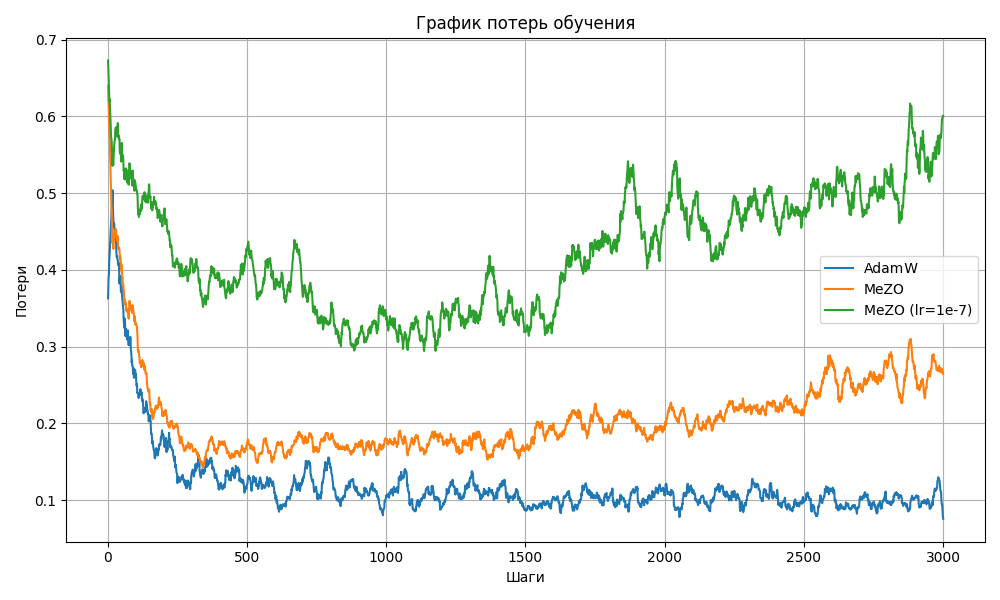
\includegraphics[width=\textwidth]{images/convergence_gap_and_instability}
    \caption{График потерь обучения для MeZO и AdamW на датасете We-Math для модели LLaVA-OneVision-Qwen2-0.5B-SI}
    \label{fig:convergence_gap}
\end{figure}

На рисунке~\ref{fig:convergence_gap} представлено сравнение графика потерь методов дообучения.

Метод MeZO демонстрирует разрыв в сходимости по сравнению с AdamW и не может достичь тех же минимальных значений потерь, что и AdamW.

Вторым важным наблюдением является нестабильность обучения при использовании MeZO.
График показывает, что потери имеют тенденцию к увеличению после начального снижения.
При этом, попытка снижения шага обучения (lr=1e-7) для MeZO не приводит к улучшению результатов.

На рискунке~\ref{fig:convergence_gap_7b} представлено сравнение графика потерь для модели LLaVA-OneVision-Qwen2-7B-SI.

\begin{figure}[H]
    \centering
    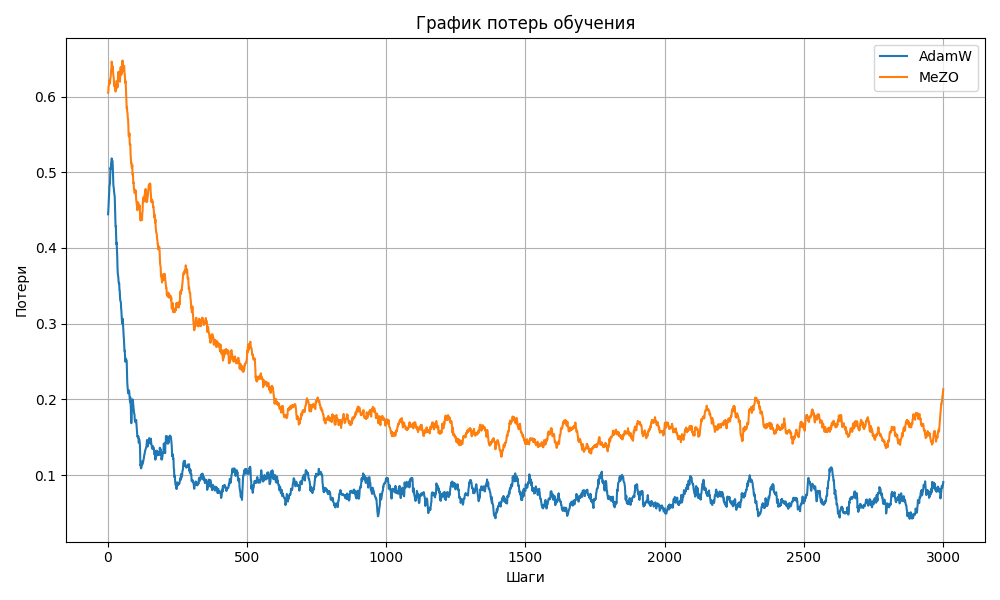
\includegraphics[width=\textwidth]{images/convergence_gap_7b}
    \caption{График потерь обучения для MeZO и AdamW на датасете We-Math для модели LLaVA-OneVision-Qwen2-7B-SI}
    \label{fig:convergence_gap_7b}
\end{figure}

Как видно из рисунка~\ref{fig:convergence_gap_7b}, разрыв в сходимости MeZO относительно AdamW сохраняется и для модели с 7B параметров.
Кроме того, заметна меньшая скорость сходимости MeZO по сравнению с моделью с 0.5B параметров.

Также был проведён эксперимент с изменением размера батча.

\begin{figure}[H]
    \centering
    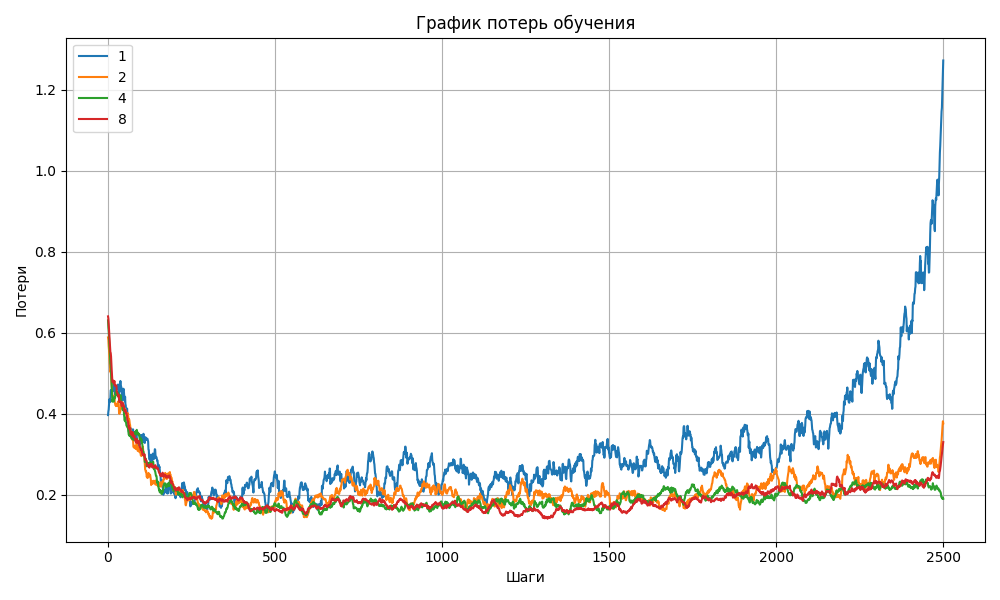
\includegraphics[width=\textwidth]{images/convergence_with_batches_full}
    \caption{График потерь обучения для MeZO на датасете We-Math с разными размерами батча для модели LLaVA-OneVision-Qwen2-0.5B-SI}
    \label{fig:convergence_with_batches}
\end{figure}

\cite{mezo-svrg} утверждает о большей нестабильности MeZO на меньших размерах батча.
На рисунке~\ref{fig:convergence_with_batches} представлено сравнение MeZO с различными размерами батча.
Как видно из рисунка, это утверждение подтверждается.
При размере батча 1 заметна сильная нестабильность и расхождение метода.
Для размера батчей выше 2 эффект становится малозаметным, но разрыв в сходимости относительно AdamW остаётся.

\section*{Выводы}

В данной главе были проведены всесторонние вычислительные эксперименты, направленные на оценку эффективности методов тонкой настройки мультимодальных моделей с использованием оптимизации нулевого порядка (метод MeZO) по сравнению с традиционным методом (AdamW).
Основные выводы, полученные в ходе экспериментов, можно сформулировать следующим образом:

\begin{itemize}
    \item \textbf{Качество дообучения.} По результатам тестирования на датасетах \textit{Br35H}, \textit{We-Math} и \textit{ChartQA} видно, что применение MeZO позволяет улучшить точность моделей относительно необученного состояния.
Однако модели, дообученные методом оптимизации нулевого порядка, могут серьёзно уступать версиям, настроенным с помощью AdamW (например, для датасета \textit{ChartQA} и модели LLaVA-OneVision-Qwen2-0.5B-SI точность MeZO составляет 28.5\% против 36.7\% при использовании AdamW).

    \item \textbf{Потребление памяти.} Одним из ключевых преимуществ метода MeZO является его крайне низкое потребление оперативной памяти.
Было показано, что использование памяти при дообучении методом MeZO соответствует режиму инференса (около 3.7 ГБ) и значительно меньше, чем при использовании AdamW (14.6 ГБ).

    \item \textbf{Сходимость и стабильность обучения.} Анализ кривых функции потерь продемонстрировал, что MeZO характеризуется менее стабильной сходимостью по сравнению с AdamW.
Наблюдался разрыв в поведении функции потерь, а параметры оптимизации оказались чувствительны к выбору гиперпараметров (таких как размер батча и шаг обучения).
Эксперименты с изменением размера батча подтвердили, что при малых размерах батча метод демонстрирует повышенную нестабильность.

    \item \textbf{Роль промпт-инжиниринга.} Дополнительный анализ показал, что качество итоговых результатов существенно зависит от корректной формулировки промпта.
\end{itemize}

\chapter*{Заключение}

В данной работе было рассмотрено применение методов оптимизации нулевого порядка для тонкой настройки мультимодальных больших языковых моделей,
что позволяет существенно снизить требования к оперативной памяти по сравнению с традиционными методами,
основанными на вычислении градиентов через обратное распространение ошибки.

Основные итоги исследования можно сформулировать следующим образом:

\begin{itemize}
    \item Был произведён анализ архитектурных решений мультимодальных моделей и подходов к тонкой настройке.

    \item Представлена теоретическая база метода SPSA и его применения для оценки градиентов без необходимости обратного распространения.
Память-эффективная версия метода (MeZO) позволяет обновлять параметры модели, используя только прямые проходы, что значительно уменьшает объём требуемой памяти.

    \item Экспериментальная часть работы включала сравнение методов оптимизации MeZO и AdamW на ряде датасетов (Br35H, We-Math, ChartQA). Результаты показали, что:
    \begin{itemize}
        \item Для более эффективного обучения MeZO требуется тщательная настройка промптов, что может быть трудоёмко и не всегда представляется возможным в реальных приложениях.
        \item Для простых датасетов по точности MeZO демонстрирует конкурентоспособные результаты, хотя и немного уступает AdamW.
        \item Для сложных задач, таких как ChartQA, MeZO показывает значительное снижение точности по сравнению с AdamW. %\item Также MeZO показывает значительное снижение точности на задачах,
        \item MeZO потребляет значительно меньше оперативной памяти, что особенно актуально при работе с крупномасштабными моделями.
        \item Сходимость метода MeZO характеризуется неустойчивостью, особенно на небольших размерах батча.
    \end{itemize}
\end{itemize}

Таким образом, хотя MeZO демонстрирует потенциал для обучения MLLM в условиях ограниченных вычислительных ресурсов,
метод требует дальнейших исследований для повышения стабильности и качества обучения.

Перспективными направлениями будущей работы для улучшение стабильности и сходимости метода MeZO
можно считать применение техник уменьшения дисперсии, адаптивной настройки гиперпараметров.
Например, в \cite{mezo} отмечалась возможность применения метода MeZO-Adam для сложных задач в качестве направления для будущих исследований.

Код, использованный во время выполнения настоящей работы, выложен в открытый доступ
на сайте GitHub и может быть воспроизведен.~\citeurl{WorkGitHub}
Также в репозиторий \texttt{LLaVA-NeXT}, на основе которого проводились эксперименты, добавлен пулл-реквест с реализацией MeZO.~\citeurl{LLaVANextPR}

%\putbibliography %Вместо этой команды будет вставлена библиография
\printbibliography

\chapter*{Приложение А}

\begin{table}[H]
\centering
\begin{tabular}{|l|l|}
\hline
\textbf{Параметр} & \textbf{Значение} \\ \hline
Vision encoder & google/siglip-so400m-patch14-384 \\ \hline
Vision tower learning rate & 1e-6 \\ \hline
MM projector type & mlp2x\_gelu \\ \hline
Vision select layer & -2 \\ \hline
Use image start/end tokens & False \\ \hline
Use image patch token & False \\ \hline
Group by modality length & True \\ \hline
Image aspect ratio & anyres\_max\_9 \\ \hline
Image grid pinpoints & (1x1),...,(6x6) \\ \hline
Patch merge type & spatial\_unpad \\ \hline
Precision & bfloat16 \\ \hline
Per device train batch size & 4 \\ \hline
Gradient accumulation steps & 1 \\ \hline
Learning rate & 1e-6 \\ \hline
Weight decay & 0.0 \\ \hline
LR scheduler type & constant \\ \hline
TF32 & False \\ \hline
Gradient checkpointing & False \\ \hline
Lazy preprocess & True \\ \hline
Torch compile & False \\ \hline
Dataloader drop last & True \\ \hline
Frames upper bound & 32 \\ \hline
\end{tabular}
\caption{Полный список общих параметров для MeZO и AdamW}
\label{app:mezo-parameters}
\end{table}

\begin{table}[H]
\centering
\begin{tabular}{|l|l|}
\hline
\textbf{Параметр} & \textbf{Значение} \\ \hline
Attention implementation & sdpa \\ \hline
Model max length & 1792 \\ \hline
\end{tabular}
\caption{Полный список общих параметров для MeZO и AdamW. Продолжение}
\label{app:mezo-parameters-2}
\end{table}

Для MeZO использовались:

\begin{table}[H]
\centering
\begin{tabular}{|l|l|}
\hline
\textbf{Параметр} & \textbf{Значение} \\ \hline
ZO epsilon & 1e-3 \\ \hline
ZO number of directions & 1 \\ \hline
\end{tabular}
\caption{Параметры MeZO}
\label{app:mezo-parameters-mezo}
\end{table}
\end{document}
